\section{Conceitos e notações}

Começamos com alguns conceitos e notações que são 
usados tanto para discretas quanto contínuas.

Em distribuições discretas, $f(x) = \Prob(X = x)$.
Em distribuições contínuas, $f(x)$ é a função densidade.

Já vimos média (\cref{eq:ch02-esperança-discreta,eq:ch02-esperança-continua}), variância (\cref{eq:ch02-def-variancia}) e momentos
(\cref{eq:ch02-def-momento}).

\begin{definition}[Moda]
    Uma \textbf{moda} de uma distribuição de uma \va\ $X$
    é um valor $x_m$ tal que $f(x_m) \ge f(x)$ para
    todo possível valor de $x$.

    Pode existir mais de uma moda.
\end{definition}

\begin{example}
    Moda em uma distribuição de uma \va\ discreta.
    \begin{center}
        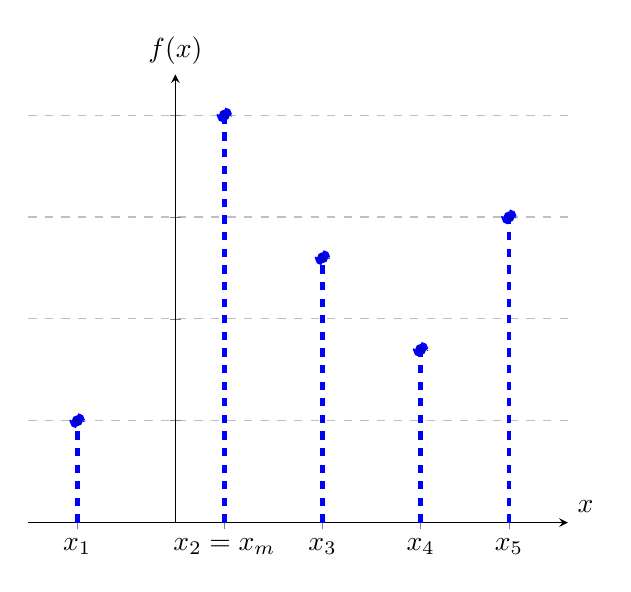
\begin{tikzpicture}
            \begin{axis}[
                unbounded coords=jump,
                ymajorgrids=true,
                major grid style={dashed},
                axis x line=middle,
                axis y line=middle,
                xmin=-3, xmax=8,
                ymin=0, ymax=4.4,
                xtick={-2, 1, 3, 5, 6.8},
                ytick={1, 2, 3, 4},
                xticklabels={
                    $x_1$, $x_2=x_m$, $x_3$, $x_4$, $x_5$
                },
                yticklabels=\empty,
                xlabel={$x$},
                ylabel={$f(x)$},
                x label style={anchor=south west},
                y label style={anchor=south},
                legend style={fill=none,draw=none},
            ]

            \addplot+[ycomb,dashed,blue,ultra thick]
                coordinates {
                    (-2, 1)
                    (1, 4)
                    (3, 2.6)
                    (5, 1.7)
                    (6.8, 3)
                };

            \end{axis}
        \end{tikzpicture}
    \end{center}
\end{example}

\begin{example}
    Moda em uma distribuição de uma \va\ contínua.
    \begin{center}
        \begin{tikzpicture}
            \begin{axis}[
                unbounded coords=jump,
                grid=major,
                major grid style={dashed},
                axis x line=middle,
                axis y line=middle,
                xmin=-3, xmax=11,
                ymin=0, ymax=0.15,
                xtick={4},
                ytick={0.133},
                xticklabels={$x_m$},
                yticklabels=\empty,
                xlabel={$x$},
                ylabel={$f(x)$},
                x label style={anchor=south west},
                y label style={anchor=south},
                legend style={fill=none,draw=none},
            ]

            \addplot[blue,ultra thick,domain=-2:10,samples=100]
                {dnormal(x, 4, 9)};

            \end{axis}
        \end{tikzpicture}
    \end{center}
\end{example}

\begin{definition}[Quantil]
    Para $0 < \alpha < 1$, definimos o quantil $q_\alpha$ como
    \begin{align}
        q_\alpha &= \min\{x: F(x) \ge \alpha \}
    \end{align}
\end{definition}

Se $F(x)$ é uma função monótona crescente,
então $q_\alpha = F^{-1}(\alpha)$. Neste caso, temos
$F(q_\alpha) = F(F^{-1}(\alpha)) = \alpha$. A \cref{fig:ch05-quantil-monotona} ilustra esta situação.

\begin{figure}[!ht]
    \centering
    \begin{tikzpicture}
        \begin{axis}[
            unbounded coords=jump,
            grid=major,
            major grid style={dashed},
            axis x line=middle,
            axis y line=middle,
            xmin=-15, xmax=30,
            ymin=0, ymax=1.1,
            xtick=\empty,
            ytick={1},
            extra x ticks={10},
            extra y ticks={0.679},
            extra x tick labels={$q_\alpha = F^{-1}(\alpha)$},
            extra y tick labels={$\alpha$},
            xlabel={$x$},
            ylabel={$F(x)$},
            x label style={anchor=west},
            y label style={anchor=south},
            legend style={fill=none,draw=none},
        ]

        \addplot[blue,ultra thick,domain=-12:28,samples=100]
            {plog(x,7,4)};

        \draw[red, fill] (10, 0.679) circle (.5ex);
        \draw[-latex, dashed, red, thick]
            (0, 0.679) -- (10, 0.679);
        \draw[-latex, dashed, red, thick]
            (10, 0.679) -- (10, 0);
            

        \end{axis}
    \end{tikzpicture}
    \caption{Quantil quando $F(x)$ é monótona crescente}
    \label{fig:ch05-quantil-monotona}
\end{figure}

\begin{example}
    Vamos observar um caso em que $F(x)$ é não-decrescente.

    \begin{center}
        \begin{tikzpicture}
            \begin{axis}[
                unbounded coords=jump,
                grid=major,
                major grid style={dashed},
                axis x line=middle,
                axis y line=middle,
                xmin=-9, xmax=36,
                ymin=0, ymax=1.1,
                xtick=\empty,
                ytick={1},
                extra x ticks={5, 11, 18},
                extra y ticks={0.119, 0.378},
                extra x tick labels={
                    $q_{\alpha_1}$, $q_{\alpha_2}$, $x^*$
                },
                extra y tick labels={$\alpha_1$, $\alpha_2$},
                xlabel={$x$},
                ylabel={$F(x)$},
                x label style={anchor=west},
                y label style={anchor=south},
                legend style={fill=none,draw=none},
            ]
    
            \addplot[blue,ultra thick,domain=-6:11,samples=100]
                {plog(x-6,7,4)};

            \addplot[blue,ultra thick,domain=11:21,samples=2]
                {0.378};

            \addplot[blue,ultra thick,domain=21:34,samples=100]
                {plog(x-16,7,4)};
    
            \draw[red, fill] (5, 0.119) circle (.5ex);
            \draw[-latex, dashed, red, thick]
                (0, 0.119) -- (5, 0.119);
            \draw[-latex, dashed, red, thick]
                (5, 0.119) -- (5, 0);

            \draw[red, fill] (11, 0.378) circle (.5ex);
            \draw[-latex, dashed, red, thick]
                (0, 0.378) -- (11, 0.378);
            \draw[-latex, dashed, red, thick]
                (11, 0.378) -- (11, 0);
                
            \draw[blue, fill] (18, 0.378) circle (.5ex);
    
            \end{axis}
        \end{tikzpicture}
    \end{center}

    Observe que os quantis $q_{\alpha_1}$e $q_{\alpha_2}$
    são dados por $F(\alpha_1)$ e $F(\alpha_2)$, respectivamente.
    No entanto, temos que $F(x^*) = \alpha_2$,
    porém $x^* > q_{\alpha_2}$.
\end{example}

\begin{example}
    $X$ é uma \va\ discreta com três valores distintos 
    ($x_1 < x_2 < x_3$).

    \begin{center}
        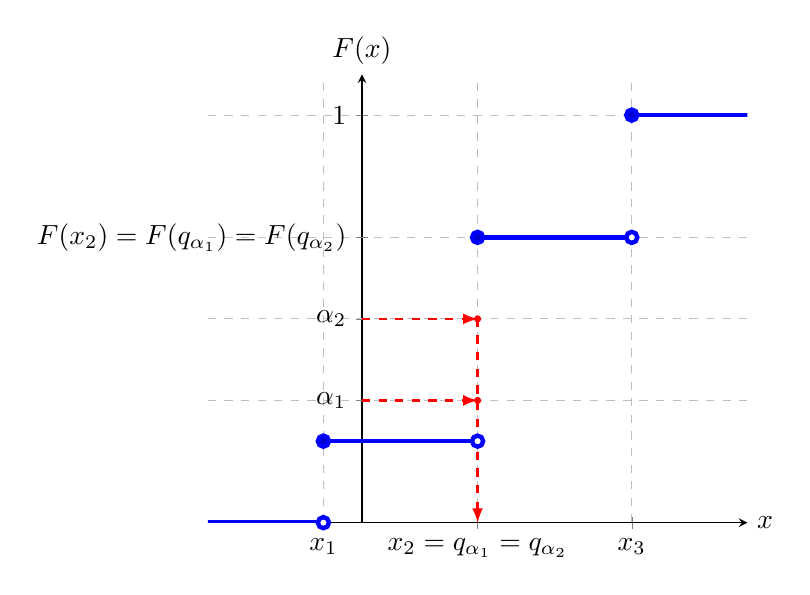
\begin{tikzpicture}[
            declare function={
            F(\x) =
                (\x>=-1) * .2 +
                (\x>=3) * .5 +
                (\x>=7) * .3
            ;}
            ]
            \begin{axis}[
                unbounded coords=jump,
                grid=major,
                major grid style={dashed},
                axis x line=middle,
                axis y line=middle,
                xmin=-4, xmax=10,
                ymin=0, ymax=1.1,
                xtick={-1, 3, 7},
                ytick={1},
                xticklabels={$x_1$,
                    $x_2 = q_{\alpha_1} = q_{\alpha_2}$, $x_3$},
                extra y ticks={0.3, 0.5, .7},
                extra y tick labels={
                    $\alpha_1$, $\alpha_2$,
                    $F(x_2) = F(q_{\alpha_1}) = F(q_{\alpha_2})$
                },
                xlabel={$x$},
                ylabel={$F(x)$},
                x label style={anchor=west},
                y label style={anchor=south},
                legend style={fill=none,draw=none},
            ]
    
            \addplot+[
                jump mark left,
                ultra thick,
                blue,
                samples at={-5, -1, 3, 7, 11}
            ] {F(x)};

            \addplot[
                only marks,
                blue,
                fill=white,
                ultra thick,
                samples at={-1, 3, 7}
            ] {F(x-0.03)};

            \draw[-latex, dashed, red, thick]
                (0, .3) -- (3, 0.3);
            \draw[red, fill] (3, 0.3) circle (.25ex);
            \draw[-latex, dashed, red, thick]
                (0, .5) -- (3, 0.5);
            \draw[red, fill] (3, 0.5) circle (.25ex);
            \draw[-latex, dashed, red, thick]
                (3, .5) -- (3, 0);
    
            \end{axis}
        \end{tikzpicture}
    \end{center}

    Neste exemplo, note que $q_{\alpha_1} = q_{\alpha_2} = x_2$,
    Mas $F(q_{\alpha_1}) > \alpha_1$, bem como
    $F(q_{\alpha_2}) > \alpha_2$.
\end{example}